\documentclass[11pt]{beamer}
\usepackage[utf8]{inputenc}
\usepackage[T1]{fontenc}

% Better hyphenation etc.
\usepackage{microtype}

% Define subfigures
\usepackage{subcaption}
\captionsetup{compatibility=false}

% Include images
\usepackage{graphicx}

% Disable navigation buttons
\beamertemplatenavigationsymbolsempty

% Hide figure caption prefix
\setbeamertemplate{caption}{\raggedright\insertcaption\par}

% Insert title pages at the beginning of a section
\AtBeginSection[]{
  \begin{frame}
  \vfill
  \centering
  \Huge{\insertsectionhead}
  \vfill
  \end{frame}
}

\begin{document}

\begin{frame}
  \begin{center}
    
\includegraphics[width=120pt]{thesis/logo}\\

    \vspace{2em}

    {\LARGE Berechnungen mit beliebig verteilten Zufallsgrößen}\\
  \end{center}
\end{frame}

\begin{frame}
  \frametitle{Das Problem}
  \begin{figure}
    \centering
    \begin{subfigure}{0.3\textwidth}
      \centering
      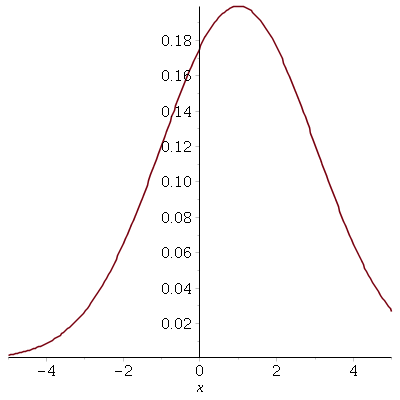
\includegraphics[width=\textwidth]{presentation/example-x}
      \caption{$X$-Modell}
    \end{subfigure}
    \hspace{4.5em}
    \begin{subfigure}{0.3\textwidth}
      \centering
      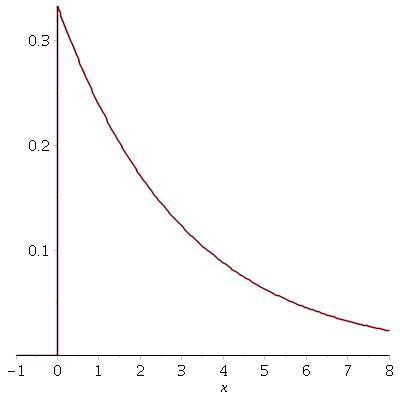
\includegraphics[width=\textwidth]{presentation/example-y}
      \caption{$Y$-Modell}
    \end{subfigure}
    \\
    \vspace{1em}
    \begin{subfigure}{0.3\textwidth}
      \centering
      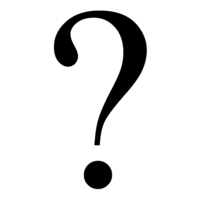
\includegraphics[width=\textwidth]{presentation/question-mark}
      \caption{$Z = f(X, Y)$}
    \end{subfigure}
  \end{figure}
\end{frame}

\begin{frame}[fragile]
  \frametitle{Die analytische Lösung}
  \begin{figure}
    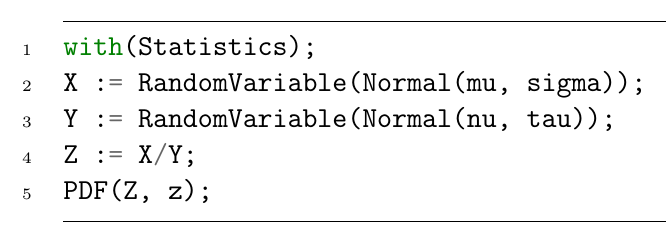
\includegraphics[width=0.8\textwidth]{presentation/maple-code}
  \end{figure}
\end{frame}

\begin{frame}
  \frametitle{Die analytische Lösung}
  \begin{figure}
    \centering
    \begin{subfigure}{0.45\textwidth}
      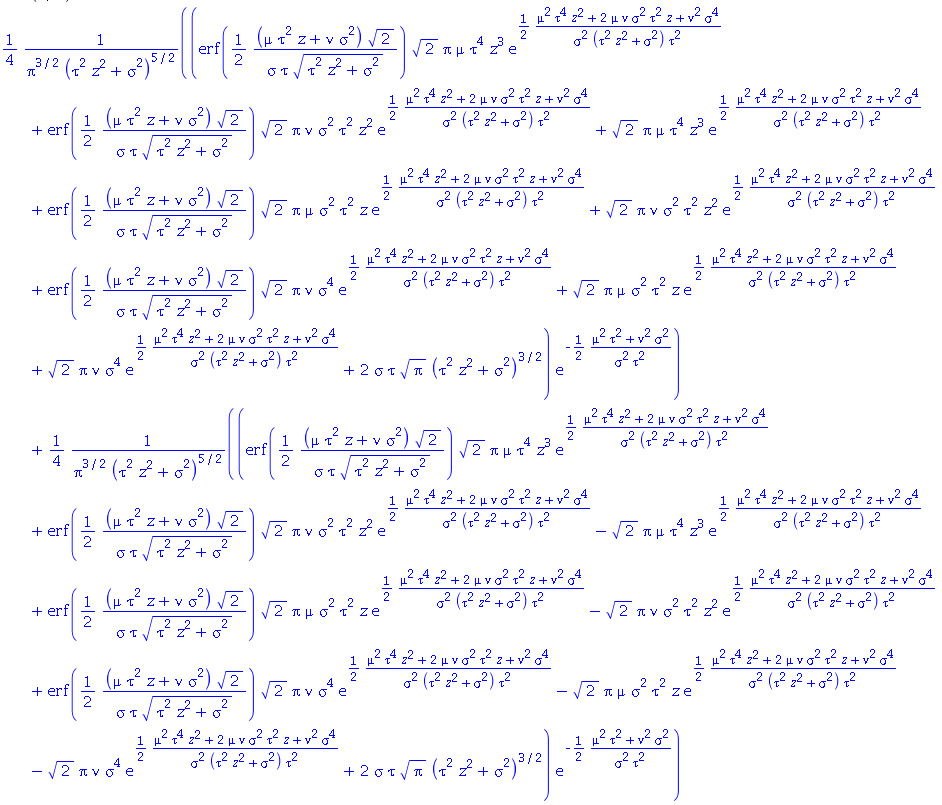
\includegraphics[width=\textwidth]{thesis/introduction/maple-pdf}
      \caption{Exakt, aber unhandlich}
    \end{subfigure}
    \hfill
    \begin{subfigure}{0.45\textwidth}
      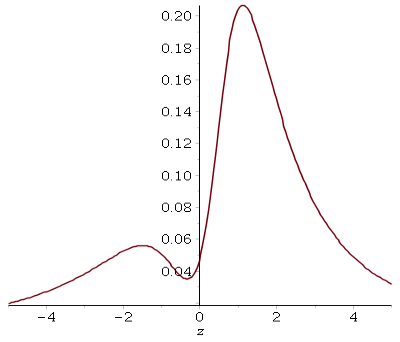
\includegraphics[width=\textwidth]{thesis/introduction/maple-plot}
      \caption{Plot der PDF von $Z$}
    \end{subfigure}
  \end{figure}
\end{frame}

\begin{frame}[fragile]
  \frametitle{Mit roher Gewalt - Sampling}
  \begin{figure}
    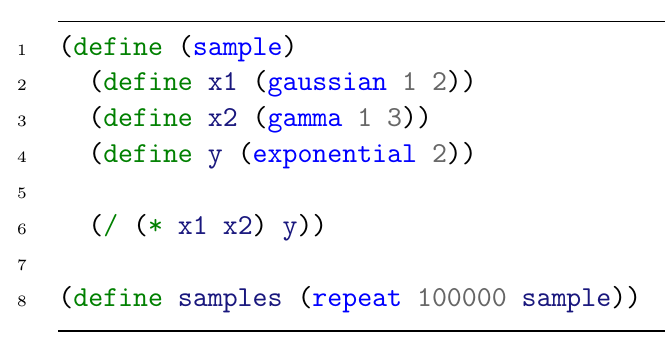
\includegraphics[width=0.8\textwidth]{presentation/church-code}
  \end{figure}
\end{frame}

\begin{frame}
  \frametitle{Mit roher Gewalt - Sampling}
  \begin{figure}
    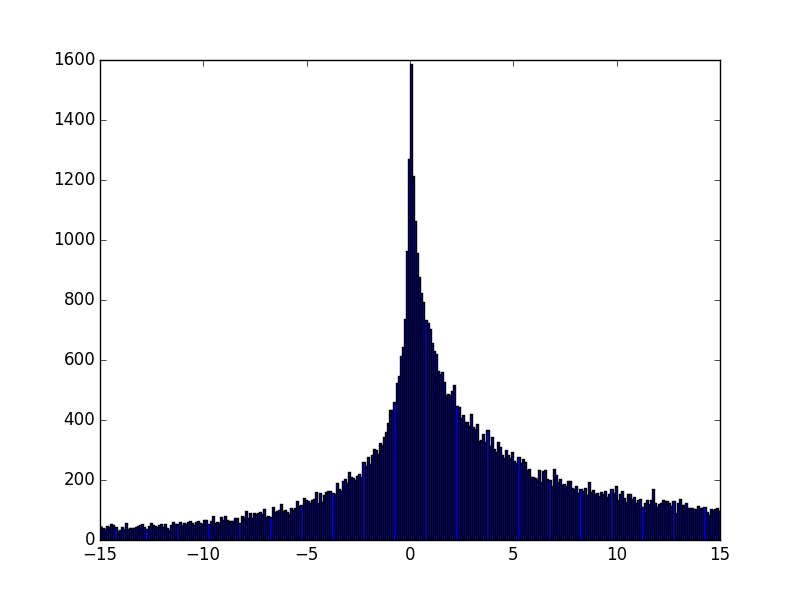
\includegraphics[width=0.8\textwidth]{thesis/introduction/church-pdf}
    \caption{Histogramm der Samples}
  \end{figure}
\end{frame}

\section{Unsere Idee}

\begin{frame}
  \frametitle{Der Wunschzettel}
  Unser Ansatz sollte
  \begin{itemize}
  \item schneller sein als analytisches Berechnen
  \item die Verteilungen in einer komprimierten Form speichern
  \item hinreichend präzise Ergebnisse liefern
  \item einfach zu benutzen sein
  \end{itemize}
\end{frame}

\begin{frame}
  \frametitle{Die Idee}
  \begin{enumerate}
  \item Alle Eingaben in eine angenehme Repräsentation umwandeln
  \item Mit dieser wird die eigentliche Rechnung durchgeführt
  \end{enumerate}
\end{frame}

\begin{frame}
  \frametitle{Gaußsche Mischverteilungen - Was ist das?}
  \begin{columns}[T]
    \begin{column}{.5\textwidth}
      \begin{figure}
        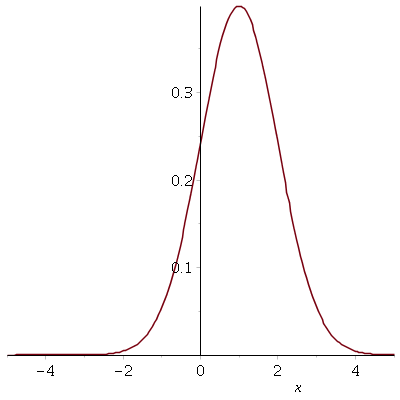
\includegraphics[width=0.8\textwidth]{presentation/mixtures-one}
      \end{figure}
      \begin{equation*}
        X \sim \mathcal{N}(\mu, \sigma)
      \end{equation*}
    \end{column}
    \begin{column}{.5\textwidth}
      \begin{figure}
        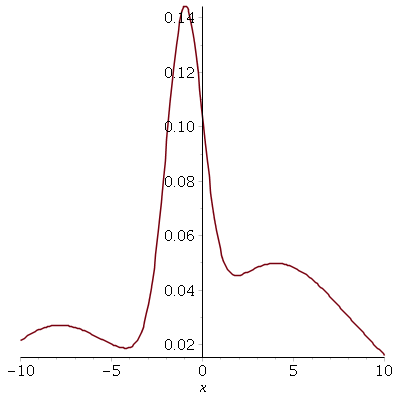
\includegraphics[width=0.8\textwidth]{presentation/mixtures-multiple}
      \end{figure}
      \begin{equation*}
        X \sim \sum_{i = 1}^{n} \alpha_{i} \mathcal{N}(\mu_{i}, \sigma_{i})
      \end{equation*}
      \begin{equation*}
        \sum_{i = 1}^{n} \alpha_{i} = 1
      \end{equation*}
    \end{column}
  \end{columns}
\end{frame}

\begin{frame}
  \frametitle{Gaußsche Mischverteilungen - Warum?}
  \begin{itemize}
  \item Beliebig genaue Approximation von Verteilungen
  \item Gaußverteilungen sind abgeschlossen bezüglich affiner Transformationen
  \end{itemize}
\end{frame}

\section{Umwandeln der Eingaben}

\begin{frame}
  \frametitle{Expectation-Maximization-Algorithmus}
  Iterativer Algorithmus, um ein Modell an Daten anzupassen
  \vspace{2em}
  \begin{enumerate}
  \item Initialisiere ein Modell mit zufälligen Parametern
  \item Verbessere die Parameter iterativ
  \end{enumerate}
\end{frame}

\begin{frame}
  \frametitle{EM - Cauchy-Verteilung}
  \begin{figure}[h]
  \centering
  \begin{subfigure}{0.45\textwidth}
    \centering
    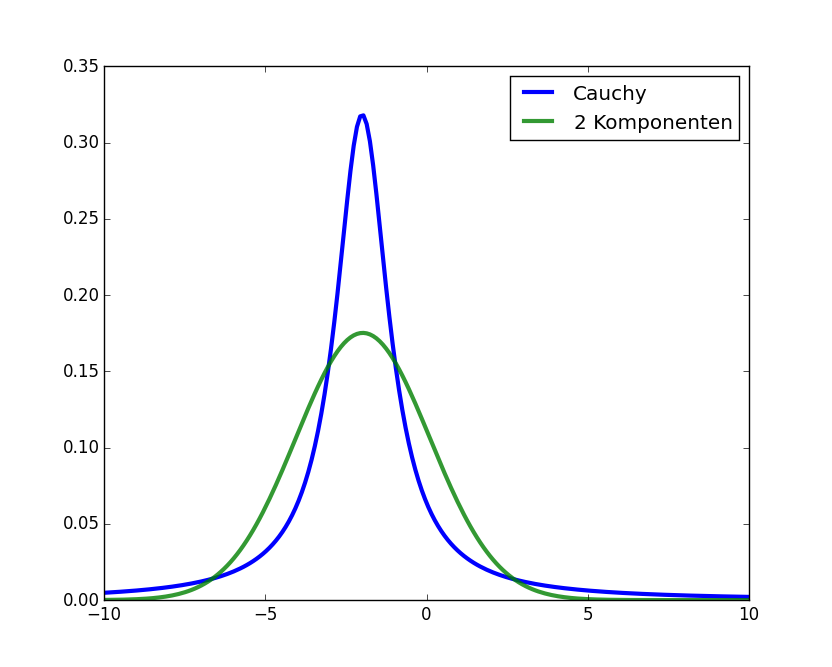
\includegraphics[width=\textwidth]{presentation/cauchy-2-components}
  \end{subfigure}
  \hfill
  \begin{subfigure}{0.45\textwidth}
    \centering
    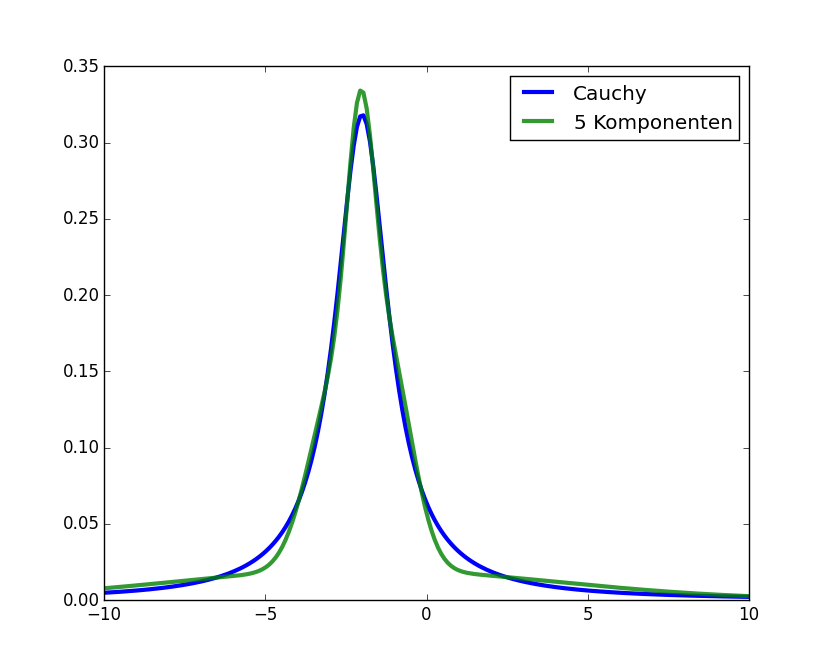
\includegraphics[width=\textwidth]{presentation/cauchy-5-components}
  \end{subfigure}
  \caption{Eine Cauchy-Verteilung kann mit wenigen Komponenten angenähert werden}
  \label{fig:em-cauchy}
\end{figure}
\end{frame}

\begin{frame}
  \frametitle{EM - Gleichverteilung}
  \begin{figure}[h]
  \centering
  \begin{subfigure}{0.45\textwidth}
    \centering
    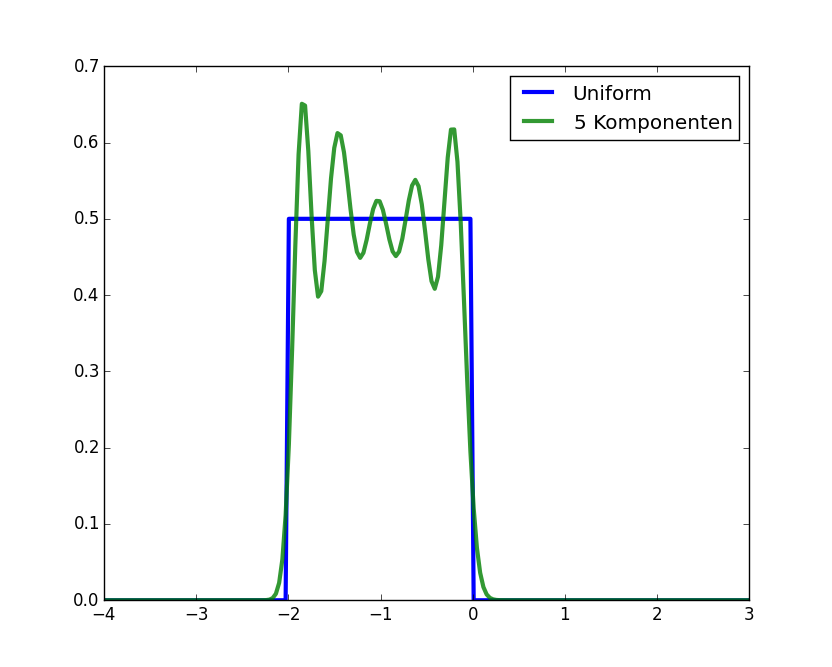
\includegraphics[width=\textwidth]{presentation/uniform-5-components}
  \end{subfigure}
  \hfill
  \begin{subfigure}{0.45\textwidth}
    \centering
    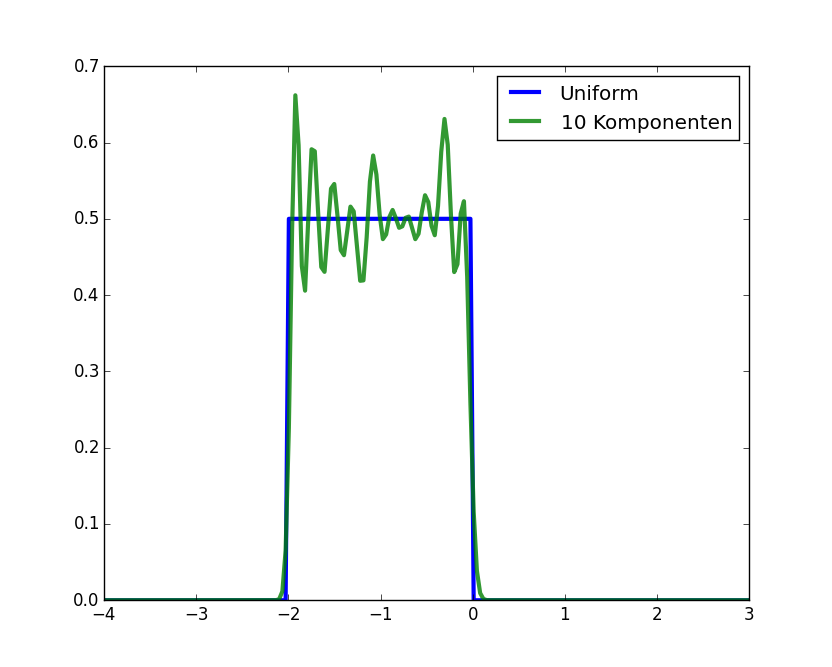
\includegraphics[width=\textwidth]{presentation/uniform-10-components}
  \end{subfigure}
  \caption{Trotz Ecken überzeugt die Approximation}
  \label{fig:em-uniform}
\end{figure}
\end{frame}

\section{Abschluss von Mischverteilungen}

\begin{frame}
  \frametitle{Das Lemma}
  \begin{equation*}
    p(X = x) = \sum_{i = 1}^{n} \alpha_{i} \cdot p(X_{i} = x) \qquad p(Y = y) = \sum_{k = 1}^{m} \beta_{k} \cdot p(Y_{k} = y)
  \end{equation*}
  \vspace{1.5em}
  \begin{lemma}
    Seien $X$ und $Y$ wie oben und
    $f : \mathbb{R} \times \mathbb{R} \rightarrow \mathbb{R}$ eine
    diffentierbare Funktion, die im ersten Argument invertierbar ist. Dann ist
    die Verteilung von $Z = f(X, Y)$ durch die folgende Gleichung gegeben.
    \begin{equation*}
      p(Z = z) = \sum_{i = 1}^{n} \sum_{k = 1}^{m} \alpha_{i} \beta_{k} p(f(X_{i}, Y_{k}) = z)
    \end{equation*}
  \end{lemma}
\end{frame}

\section{Abschluss von Gaußverteilungen}

\begin{frame}
  \frametitle{Affine Transformationen und Summen}

  {\Large Affine Transformationen}\\
  \vspace{1em}
  Seien $X \sim \mathcal{N}(\mu, \sigma^{2})$ und
  $\alpha \in \mathbb{R} \setminus \{ 0 \}$ und $\beta \in \mathbb{R}$.
  \begin{equation*}
    \alpha X + \beta \sim \mathcal{N}(\alpha \mu + \beta, \alpha^{2}\sigma^{2})
  \end{equation*}

  \vspace{3em}

  {\Large Summen von Gaußverteilten Variablen}\\
  \vspace{1em}
  Seien $X \sim \mathcal{N}(\mu, \sigma^{2})$ und $Y \sim \mathcal{N}(\nu, \tau^{2})$
  \begin{equation*}
    X + Y \sim \mathcal{N}(\mu + \nu, \sigma^{2} + \tau^{2})
  \end{equation*}
\end{frame}

\begin{frame}
  \frametitle{Affine Transformationen in mehreren Variablen}

  \begin{equation*}
    f(a, b, c) = \frac{3a}{5} + 2b - c - 3
  \end{equation*}

  \begin{figure}
    \centering
    \begin{subfigure}[t]{0.45\textwidth}
      \centering
      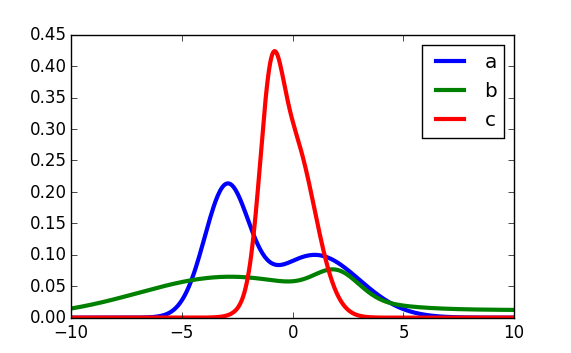
\includegraphics[width=\textwidth]{thesis/operations/affine-vars}
      \caption{Variablen mit unterschiedlichen Verteilungen}
    \end{subfigure}
    \hfill
    \begin{subfigure}[t]{0.45\textwidth}
      \centering
      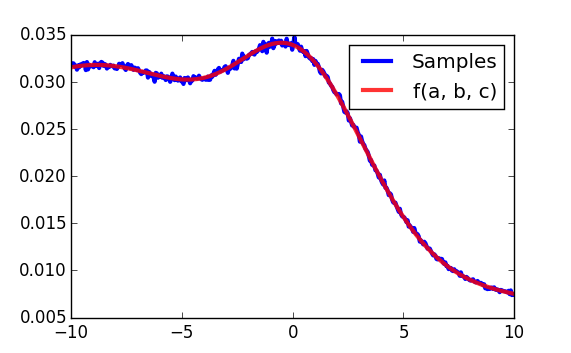
\includegraphics[width=\textwidth]{thesis/operations/affine-result}
      \caption{Die Verteilung von $f(a, b, c)$ wird exakt berechnet}
    \end{subfigure}
  \end{figure}
\end{frame}

\section{Multiplikation und Division}

\begin{frame}
  \frametitle{Multiplikation von Gaußschen Zufallsvariablen}

  Seien $X \sim \mathcal{N}(\mu, \sigma^{2})$,
  $Y \sim \mathcal{N}(\nu, \tau^{2})$ und $Z = X \cdot Y$. \vfill
  Zu lösendes Integral
  \begin{equation*}
    p(Z = z) = \int_{-\infty}^{\infty} \frac{1}{|y|} \cdot \mathcal{N}\left( \frac{z}{y} \mid \mu, \sigma^{2} \right) \cdot \mathcal{N}(y \mid \nu, \tau^{2})~\mathrm{d}y
  \end{equation*}
  \vfill
  Gauß-Hermite-Approximation mit $n$ Stützstellen
  \begin{equation*}
    p(Z = z) \approx \sum_{i = 1}^{n} \frac{w_{i}}{\sqrt{\pi}} \cdot \mathcal{N}\left( z \mid \left(\sqrt{2 \tau^{2}} x_{i} + \nu\right)\mu, \left(\sqrt{2 \tau^{2}} x_{i} + \nu\right)^{2}\sigma^{2} \right)
  \end{equation*}
\end{frame}

\begin{frame}
  \frametitle{Multiplikation - Demo}

  \begin{figure}
    \centering
    \begin{subfigure}[t]{0.45\textwidth}
      \centering
      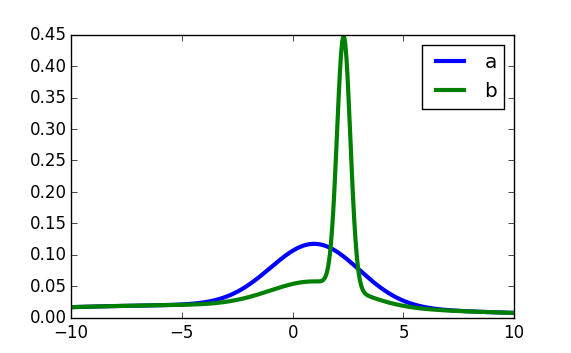
\includegraphics[width=\textwidth]{thesis/operations/product-hermite-vars}
      \caption{Die Variablen}
    \end{subfigure}
    \hfill
    \begin{subfigure}[t]{0.45\textwidth}
      \centering
      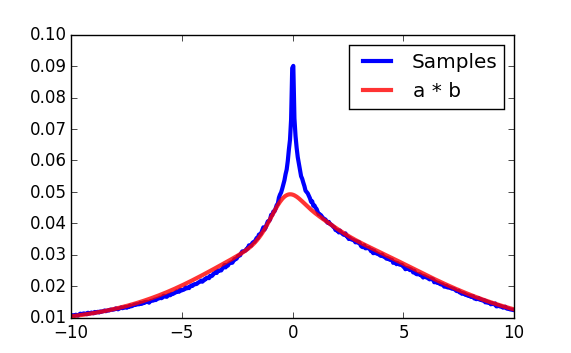
\includegraphics[width=\textwidth]{thesis/operations/product-hermite-50-components}
      \caption{$300$ Komponenten}
    \end{subfigure}
  \end{figure}
  \begin{figure}
    \centering
    \begin{subfigure}[t]{0.45\textwidth}
      \centering
      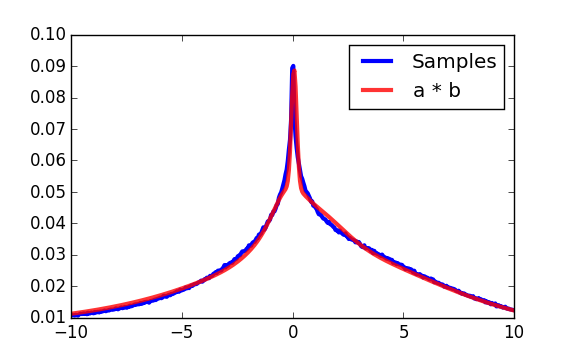
\includegraphics[width=\textwidth]{thesis/operations/product-hermite-100-components}
      \caption{600 Komponenten}
    \end{subfigure}
    \hfill
    \begin{subfigure}[t]{0.45\textwidth}
      \centering
      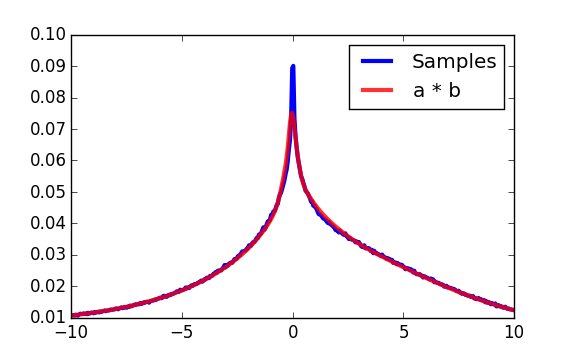
\includegraphics[width=\textwidth]{thesis/operations/product-hermite-2000-components}
      \caption{12000 Komponenten}
    \end{subfigure}
  \end{figure}
\end{frame}

\begin{frame}
  \frametitle{Division von Gaußschen Zufallsvariablen}

  Seien $X \sim \mathcal{N}(\mu, \sigma^{2})$,
  $Y \sim \mathcal{N}(\nu, \tau^{2})$ und $Z = X / Y$. \vfill
  Zu lösendes Integral
  \begin{equation*}
    p(Z = z) = \int_{-\infty}^{\infty} |y| \cdot \mathcal{N}\left( zy \mid \mu, \sigma^{2} \right) \cdot \mathcal{N}(y \mid \nu, \tau^{2})~\mathrm{d}y
  \end{equation*}
  \vfill
  Gauß-Hermite-Approximation mit $n$ Stützstellen
  \begin{equation*}
    p(Z = z) \approx \sum_{i = 1}^{n} \frac{w_{i}}{\sqrt{\pi}} \cdot \mathcal{N}\left( z \left| \frac{\mu}{\sqrt{2 \tau^{2}} x_{i} + \nu}, \frac{\sigma^{2}}{\left(\sqrt{2 \tau^{2}} x_{i} + \nu\right)^{2}} \right.\right)
  \end{equation*}
\end{frame}

\begin{frame}
  \frametitle{Division - Demo}

  \begin{figure}
    \centering
    \begin{subfigure}[t]{0.45\textwidth}
      \centering
      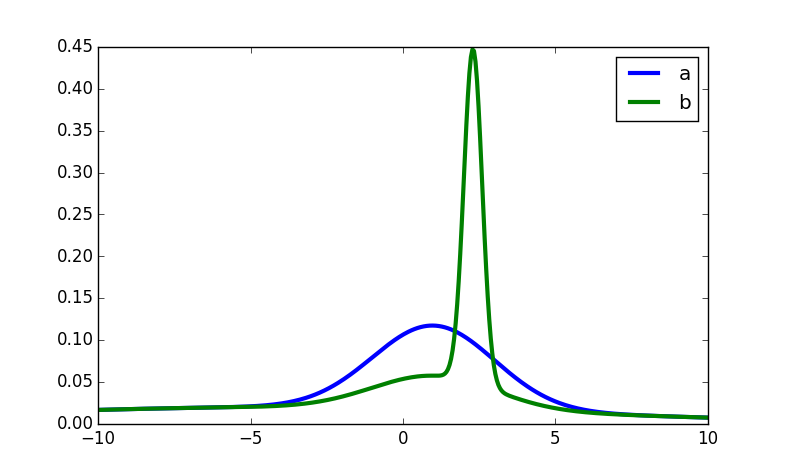
\includegraphics[width=\textwidth]{thesis/operations/quotient-vars}
      \caption{Die Variablen}
    \end{subfigure}
    \hfill
    \begin{subfigure}[t]{0.45\textwidth}
      \centering
      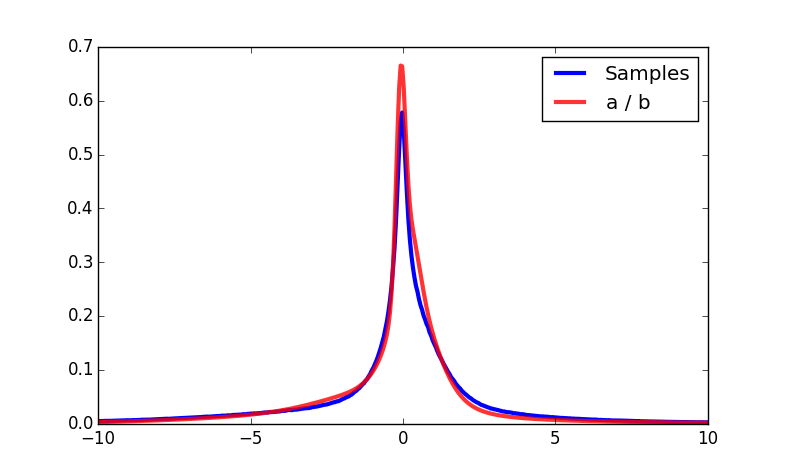
\includegraphics[width=\textwidth]{thesis/operations/quotient-2-components}
      \caption{$12$ Komponenten}
    \end{subfigure}
  \end{figure}
\end{frame}

\section{Evaluation}

\begin{frame}
  \frametitle{Der Wunschzettel}
  Unser Ansatz sollte
  \begin{itemize}
  \item schneller sein als analytisches Berechnen
  \item die Verteilungen in einer komprimierten Form speichern
  \item hinreichend präzise Ergebnisse liefern
  \item einfach zu benutzen sein
  \end{itemize}
\end{frame}

\begin{frame}
  \frametitle{Komplexes Beispiel - Code}
  \begin{figure}
    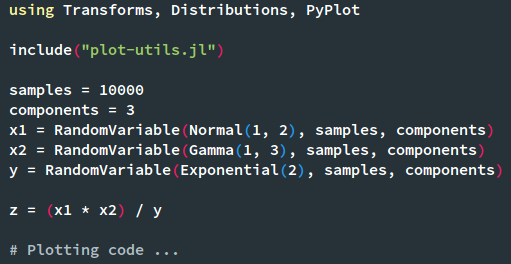
\includegraphics[width=0.8\textwidth]{presentation/code}
  \end{figure}
\end{frame}

\begin{frame}
  \frametitle{Komplexes Beispiel - Plots}
  \vspace{-0.5em}
  \begin{figure}
    \centering
    \begin{subfigure}[t]{0.3\textwidth}
      \centering
      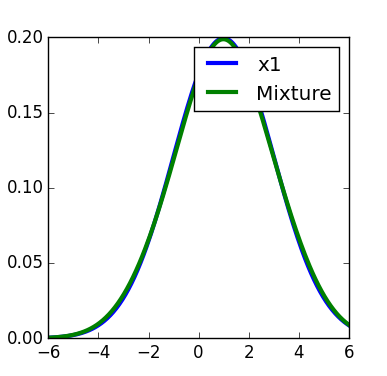
\includegraphics[width=\textwidth]{thesis/complex/introduction-var-x1}
      \caption{Gaußverteilung}
    \end{subfigure}
    \hfill
    \begin{subfigure}[t]{0.3\textwidth}
      \centering
      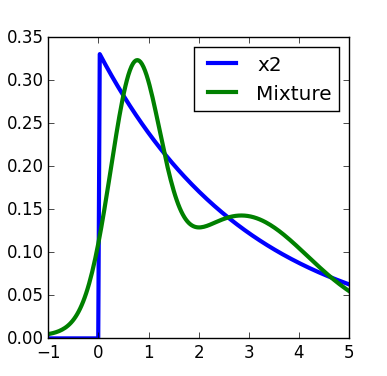
\includegraphics[width=\textwidth]{thesis/complex/introduction-var-x2}
      \caption{Gammaverteilung}
    \end{subfigure}
    \hfill
    \begin{subfigure}[t]{0.3\textwidth}
      \centering
      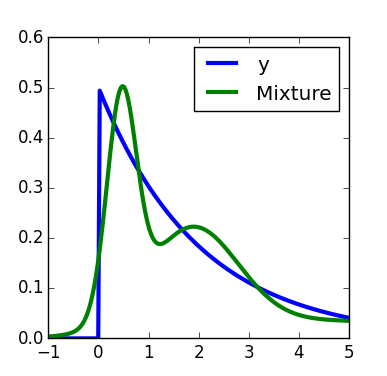
\includegraphics[width=\textwidth]{thesis/complex/introduction-var-y}
      \caption{Exponential-verteilung}
    \end{subfigure}
  \end{figure}
  \vspace{-1.5em}
  \begin{figure}
    \centering
    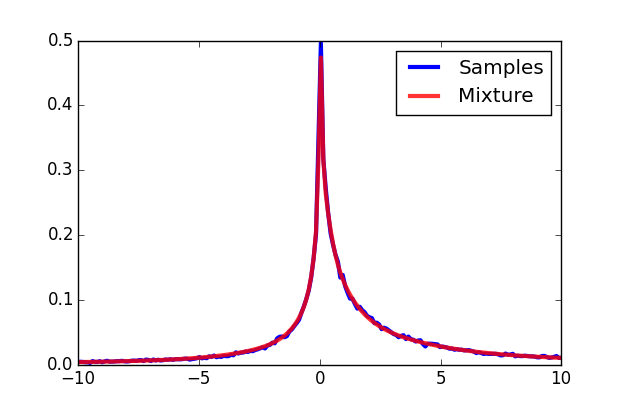
\includegraphics[width=0.5\textwidth]{thesis/complex/introduction-result}
    \caption{Die Verteilung von $Z$}
  \end{figure}
\end{frame}

\begin{frame}
  \frametitle{Einschränkungen \& offene Fragen}
  \begin{itemize}
  \item Eingaben müssen unabhängig sein
  \item Mehr Funktionen?
  \item Andere Komponentenverteilungen?
  \item Anzahl der Komponenten limitieren?
  \end{itemize}
\end{frame}

\begin{frame}
  \vfill
  \begin{center}
    \Huge{Fragen?}
  \end{center}
  \vfill
\end{frame}

\end{document}